\chapter{Quantum Relational Dynamics of JC Model
\label{chap5:RDQ_JCM_chap}}

In \refchap{chap:braun_briggs_jaynes}, we delved into the semi-classical approach to derive the Time-Dependent Schrödinger Equation (TDSE) governing the Jaynes-Cummings model. 
This method assumes a semiclassical (WKB-like) wave function for the field mode. However, 
this approach inherits the concept of ``time" as a purely classical parameter, thereby compromising its deeper and more fundamental nature.

In contrast, in \ref{chap:sebgem_Rel}, we presented a purely quantum framework to describe the dynamics of the general interacting system. Here, ``time" 
emerges as a symmetry parameter stemming from the principle of global invariance of the global energy 
eigenstate of total Hamiltonian.

This chapter explores the Jaynes-Cummings model from the perspective of Quantum Relational Dynamics. 
We aim to scrutinize the transition from a purely quantum system to semi-classical regimes, 
as previously discussed in \refchap{chap:braun_briggs_jaynes}, and to juxtapose the dynamics as 
characterized by the two distinct approaches. We demonstrate that, under appropriate limits
(consistent with the semi-classical treatment), the two approaches yield identical results. 
%Interestingly, the analysis also hints at the presence of a superselection rule.

We assume our Hamiltonian to be of the form

\begin{eqnarray}
        \label{eq:chap5_JCM_Hamiltonian}
        \oper{H} = \frac{\hbar \omega_0}{2} \oper{\sigma}_z + \hbar \omega \left(\oper{a}^\dagger \oper{a} + \frac{1}{2}\right) 
        + \hbar g \oper{\sigma}_x\left(\oper{a} + \oper{a}^\dagger\right). 
\end{eqnarray}


Under dipole-approximation and rotating-wave approximation~\cite[Chap 2]{Bina_JC_tutorial} the Hamiltonian can be written as
\begin{equation}
        \label{eq:chap5_JCM_Hamiltonian_RWA}
        \oper{H} = \frac{\hbar \omega_0}{2} \oper{\sigma}_z + \hbar \omega \left(\oper{a}^\dagger \oper{a} + \frac{1}{2}\right) 
        + \hbar g \left(\oper{\sigma}_+ \oper{a} + \oper{\sigma}_- \oper{a}^\dagger\right).
\end{equation}

\section[Exact Energy Eigenstate of JC-Hamiltonian]{Exact Energy Eigenstate of JC-Hamiltonian (resonant case)}

In the specific scenario of the Hamiltonian in Equation \ref{eq:chap5_JCM_Hamiltonian_RWA}, when 
\(\omega  = \omega_0\), known as the 
``resonance case," the system becomes exactly solvable.
This model is characterized by the Hamiltonian operator\footnote{Here, we dropped the \(1/2\) term from \(H_c\), 
simplifying calculations. This adjustment doesn't affect our analysis.}
\begin{equation}
        \label{eq:chap5_JCM_Hamiltonian_resonance}
        \oper{H} = \frac{\hbar\omega}{2} \oper{\sigma}_z + \hbar \omega \oper{a}^\dagger \oper{a}
        + \hbar g \left(\oper{\sigma}_+ \oper{a} + \oper{\sigma}_- \oper{a}^\dagger\right). 
\end{equation}
Here, it portrays the resonant interaction between two energy levels of an atom and a single mode within a cavity.
To investigate the dynamics of the JC-model, we initially aim to determine the evolution operator 
$U(t) = e^{-i t H/\hbar}$ through the diagonalization of $H$. If we achieve an eigenvalue decomposition 
$H = \sum_k a_k \lvert a_k \rangle \langle a_k \rvert$, it follows that:

\begin{equation}
U(t) = \sum_k e^{-i t a_k/\hbar} \lvert a_k \rangle \langle a_k \rvert
\end{equation}

Finding such an eigenvalue decomposition is not trivial, particularly in this context, 
given the infinite-dimensional nature of the underlying Hilbert space. However, the 
JC-Hamiltonian possesses a notably simple structure as it is block-diagonal with respect 
to the $\ket{\pm, n}$-basis. The diagonalization of the JC-Hamiltonian in 
\refeq{eq:chap5_JCM_Hamiltonian_resonance} is given in \refapp{appen:chap5_JC_calculations} .
Once you diagonalize the Hamiltonian, the eigenvalues and eigenvectors of the JC-Hamiltonian are given by
\begin{equation}
        \label{eq:chap5_JCM_eigenvalues}
        E_{\pm, n} = \hbar \omega \left(n - \frac{1}{2}\right) \pm \hbar g \sqrt{n + 1},
\end{equation}
and the corresponding eigenvectors are
\begin{equation}
        \label{eq:chap5_JCM_eigenvectors}
        \ket*{\pm, n} = \frac{1}{\sqrt{2}} \left(\ket*{g, n} \pm \ket*{e, n-1}\right).
\end{equation}
\section{Unitary Evolution operator for semiclassical JC Hamiltonian}
We discussed the coherent state-based semiclassical approximation in Chapter 
\ref{chap:braun_briggs_jaynes}, where the final result simply involved replacing 
the field operators, i.e., \( \oper{a} \) and \( \oper{a}^\dagger \), with their 
expectation values. Following a similar approach, we assume the semiclassical form 
of the Hamiltonian in Equation \ref{eq:chap5_JCM_Hamiltonian_resonance} as

\begin{equation}
    \label{eq:chap5_JCM_Hamiltonian_semi}
    \begin{aligned}
        \oper{H}_{\text{semi}} = \frac{\hbar\omega}{2} \oper{\sigma}_z + \hbar \omega \langle \oper{a}^\dagger \oper{a} \rangle
    + \hbar g \left( \oper{\sigma}_+ \langle \oper{a} \rangle + \oper{\sigma}_- \langle \oper{a}^\dagger \rangle \right),\\
    = \frac{\hbar\omega}{2} \oper{\sigma}_z + \hbar \omega N 
    + \hbar g \alpha\left( \oper{\sigma}_+ e^{-it\omega} + \oper{\sigma}_- e^{it\omega} \right),
    \end{aligned}
\end{equation}
where \(\langle a(t) \rangle = \alpha e^{-i\omega t}\). This leads to the evolution operator being expressed as
\begin{align}
        \tilde{U}(t) &= 
                \cos(\Omega t) \left(e^{-i t \omega \frac{1}{2}}\ket{+}\bra{+} + 
                e^{i t \omega \frac{1}{2}}\ket{-}\bra{-} \right)  \nonumber\\
                &- i \sin(\Omega t)
                 \left( e^{-i t \omega \frac{1}{2}}\ket{+}\bra{-}
                + e^{i t \omega \frac{1}{2}}\ket{-}\bra{+}\right)
\end{align}
where \(\Omega = {g\alpha}\). We justify the 
use of~\refeq{eq:chap5_JCM_Hamiltonian_semi} as our semi-classical Hamiltonian in~\refapp{appen:chap5_JC_calculations} . 

\begin{figure}[!h]
        \label{fig:chap5_JCM_semi_vs_quant}
        \centering
        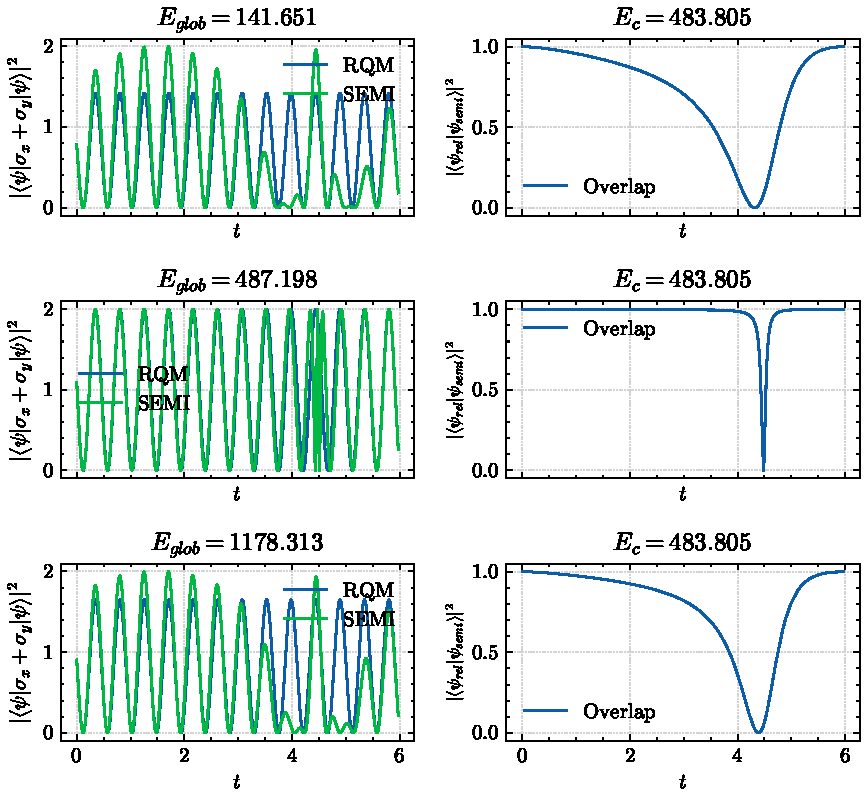
\includegraphics{chap5/semi_vs_quant.pdf}
        \caption[Expectation Value Comparison for Semi-Classical and
         Quantum Relational Dynamics]{Expectation Value Comparison 
         for Semi-Classical and Quantum Relational Dynamics. The $N_{\mathrm{cutoff}}=1000$ is taken for above calculations.}
\end{figure}
\begin{figure}[!h]
        \label{fig:chap5_JCM_overlap_avg}
        \centering
        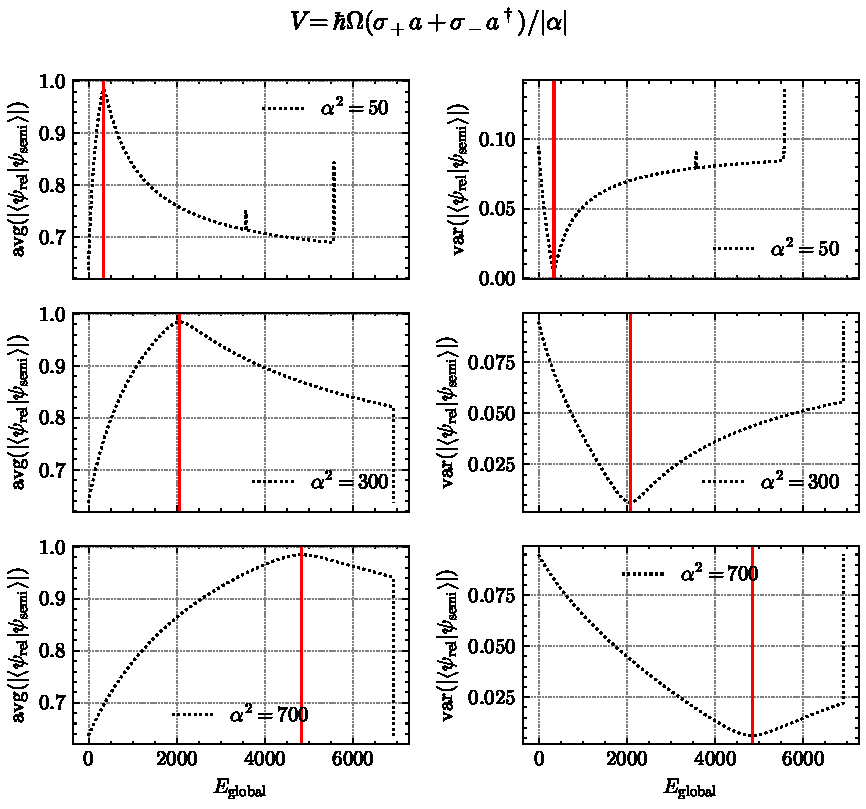
\includegraphics{chap5/overlap_average.pdf}
        \caption[Average $\abs*{\braket*{\psi_{rel}}{\psi_{semi}}}^2$ 
        (\& variance $\abs*{\braket*{\psi_{rel}}{\psi_{semi}}}^2$)
         v/s Global Eigen Energy]{The $N_{\mathrm{cutoff}}=1000$ is taken for above calculations.
         The plots shows the average $\abs*{\braket*{\psi_{rel}}{\psi_{semi}}}^2$ and 
         variance $\abs*{\braket*{\psi_{rel}}{\psi_{semi}}}^2$ over \([0, 4\pi]\) time domain 
         v/s corresponding global eigenenergy.
         Coupling \(g = \Omega / \abs*{\alpha}\) for a fixed \(\Omega\)}
\end{figure}

In \reffig{fig:chap5_JCM_semi_vs_quant}, we compare the expectation values of the operator 
\(\oper{\sigma}_x + \oper{\sigma}_y\)  for three different global energy eigenstates at a fixed 
\(E_c(\alpha^2) = \hbar \omega \abs*{\alpha}^2\). The initial state is \(N\innerGlob{\alpha}{\Psi_{E_{glob}}}\), where $N$ denotes normalization, 
for the semiclassical time evolution. We observe that both semiclassical and quantum relational dynamics exhibit 
good agreement for values of $E_{glob}$​ close to $E_c$​, indicating a scenario where ``all" the energy of the system 
is carried by the environment.

Furthermore, \reffig{fig:chap5_JCM_overlap_avg} illustrates the average of the overlap 
\(\abs*{\braket*{\psi_{rel}}{\psi_{semi}}}^2\) 
 and its variance over the time domain 
 \([0, 4\pi]\) for three different values of $E_c(\alpha^2)$ (depicted as red vertical lines). 
Here, \(\alpha^2 = \lvert n \rvert\). We observe that the average overlap is maximized for relational states 
where the energy eigenvalue of the global eigenket closely matches the energy of the semiclassical 
environment. Additionally, as we increase the average photon number, the agreement improves for 
higher energy eigenstates. These numerical findings align with the conditions outlined for an 
environment to be treated classically, as discussed in \refchap{chap:braun_briggs_jaynes} and 
\refchap{chap:briggs_rost_semiclassic}.


